\documentclass{article}

\usepackage{html}
\usepackage{graphicx}
\usepackage{tikz}

\usetikzlibrary[arrows.meta,backgrounds,calc,fit,positioning]

% Also ****ing broken.
%\newenvironment{ezcode}{\begin{quote}\begin{verbatim}}{\end{verbatim}\end{quote}}

\begin{document}

This page contains links to writings about topics such as technology, video games, and philosophy.

\tableofchildlinks*

% Tux in Minetest
% DotA2 video capture

% Internet Security and the Technocracy
% X.509
% Facebook targeting children

% Adding Certificate Revocation Lists (CRLs) to an Existing OpenSSL Implementation.
\section{2017-09-22 Adding Certificate Revocation Lists (CRLs) to an Existing OpenSSL Implementation}
I recently took it upon myself to add Certificate Revocation List (CRL) functionality to an SSL-enabled program (\htmladdnormallink{InspIRCd}{https://github.com/inspircd/inspircd/pull/1370}).  This blog details both the code that I used and some unexpected functionality regarding how CRLs behave.  Hopefully this blog will prove useful to someone else who needs to tread this path.

\subsection{Code Itself}
The code itself is actually quite simple, consisting of two basic steps: loading the CRL files and then enabling CRL checking.  In order to load the CRL files, begin by getting the \texttt{X509_STORE *} from the \texttt{SSL_CTX *} by calling \texttt{SSL_CTX_get_cert_store(3)}, then load the CRL files into the \texttt{X509_STORE *} by calling \texttt{X509_STORE_load_locations()} with the specified CRL file and path locations.  The definition of the functions can be found in \texttt{openssl/x509_vfy.h} in your system's include file directory.  The code looks something like:
\begin{quote}
\begin{verbatim}
	SSL_CTX *ctx = sslctx; // Defined elsewhere.
	X509_STORE *store;
	char *crlfile = "/path/to/single/file.pem";
	char *crlpath = "/path/to/entire/directory";

	if (!(store = SSL_CTX_get_cert_store(ctx))) {
		fprintf(stderr, "No cert store found\n");
		return -1;
	}
	if (!X509_STORE_load_locations(store, crlfile, crlpath)) {
		fprintf(stderr, "Unable to load CRL files\n");
		return -1;
	}
\end{verbatim}
\end{quote}
This will load the CRL files, but will not enable CRL checking; this has to be done by setting a flag value in the \texttt{X509_STORE *}.  There at least two possible options: one is to check only the leaf certificate, the other is to check all certificates in the chain.  The former option can be accomplished by setting only \texttt{X509_V_FLAG_CRL_CHECK} while the latter can be accomplished by setting two flags \texttt{X509_V_FLAG_CRL_CHECK | X509_V_FLAG_CRL_CHECK_ALL}.  The latter option (the entire chain) is almost certainly what you want.
\begin{quote}
\begin{verbatim}
	char* crlmode; // Defined elsewhere.
	int crlflags;

	if (!strcmp(crlmode, "chain")) {
		crlflags = X509_V_FLAG_CRL_CHECK | X509_V_FLAG_CRL_CHECK_ALL;
	} else if (!strcmp(crlmode, "leaf")) {
		crlflags = X509_V_FLAG_CRL_CHECK;
	} else {
		fprintf(stderr, "Unknown flag mode '%s'\n", crlmode);
		return -1;
	}
	if (X509_STORE_set_flags(store, crlflags) != 1) {
		fprintf(stderr, "Unable to set flags\n");
		return -1;
	}
\end{verbatim}
\end{quote}
\ldots and that's it!  CRLs should now be enabled for your program.  However, do not rest easily just yet, as CRLs offer several pitfalls for the unwary, as detailed below.

\subsection{Missing CRL Files}
Consider the following, simple certificate chain:
\begin{center}
\begin{figure}
\begin{makeimage}
\fbox{
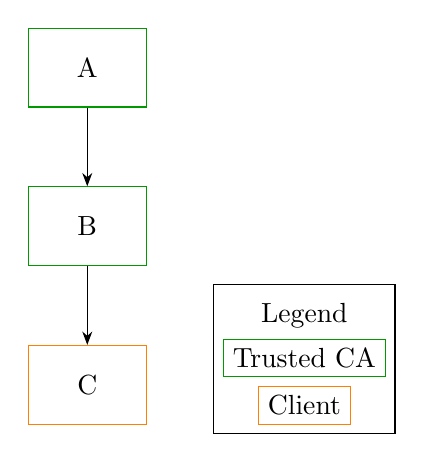
\begin{tikzpicture}
	% Styles.
	[ca/.style={rectangle,draw=green!60!black,minimum height=1cm,minimum width=1.5cm},
	leaf/.style={rectangle,draw=orange,minimum height=1cm, minimum width=1.5cm}]
	% Certificates.
	\node (A) at (0, 0) [ca] {A};
	\node (B) [below=of A] [ca] {B};
	\node (C) [below=of B] [leaf] {C};
	\draw[-Stealth] (A) -- (B);
	\draw[-Stealth] (B) -- (C);
	% Legend.
	\node (lanchor) at ($(current bounding box.south east) + (2, 0)$) {};
	\node (legend) at (lanchor) [above=1.1cm] {Legend};
	\node (l1) at (lanchor) [above=0.6cm,draw=green!60!black] {Trusted CA};
	\node (l2) at (lanchor) [above=0.0cm,draw=orange] {Client};
	\node [rectangle,draw,fit=(legend) (l1) (l2)] {};
\end{tikzpicture}
}
\end{makeimage}
\caption{Simple certificate chain, where A and B are CAs and C is the client.}
\end{figure}
\end{center}
The server trusts Certificate Authorities (CAs) A and B to issue valid certificates, thus C's certificate will be accepted.  Without CRLs this scenario will work as expected, C will be able to connect to the server without a problem.  Now, assume that the server enables CRLs, generates a CRL for A, and then configures itself to use A's CRL; a CRL for B is not generated as B has not revoked any certificate and thus there doesn't \emph{seem} to be any need to generate a CRL for B.  As you can probably guess by now, C will not be able to connect in this scenario, because the default CRL-checking method requires \emph{every} CA in the chain to have a CRL file loaded, thus C cannot connect unless both A \emph{and} B generate CRL files, \emph{even if they have no revoked certificates}.
\begin{center}
\begin{figure}
\begin{makeimage}
\fbox{
\begin{tikzpicture}
	% Styles.
	[ca/.style={rectangle,draw=green!60!black,minimum height=1cm,minimum width=1.5cm},
	leaf/.style={rectangle,draw=red,minimum height=1cm, minimum width=1.5cm},
	x/.pic={
		\draw[--] (-1mm,1mm) -- (1mm,-1mm);
		\draw[--] (-1mm,-1mm) -- (1mm,1mm);
	}]
	% Certificates.
	\node (A) at (0, 0) [ca] {A};
	\node (B) [below=of A] [ca] {B};
	\node (C) [below=of B] [leaf] {C};
	\draw[-Stealth] (A) -- (B);
	\draw[-Stealth] (B) -- (C)
		node[pos=0.5](fail){}
		pic [pos=0.5,red] {x};
	\node (error) [right=of fail] {No CRL file for B};
	\draw[-Stealth] (error) -- (fail);
	% Legend.
	\node (lanchor) at ($(current bounding box.south east) + (1.5, 0)$) {};
	\node (legend) at (lanchor) [above=1.1cm] {Legend};
	\node (l1) at (lanchor) [above=0.6cm,draw=green!60!black] {Trusted CA};
	\node (l2) at (lanchor) [above=0.0cm,draw=red] {Client};
	\node [rectangle,draw,fit=(legend) (l1) (l2)] {};
\end{tikzpicture}
}
\end{makeimage}
\caption{Each CA is required to have a CRL file.}
\end{figure}
\end{center}

The consequence of this is that enabling CRL-checking requires gathering CRL files, a task that is likely non-trivial.  The alternative is to override OpenSSL's verify callback by defining your own verify function and then telling OpenSSL to use said function with \texttt{X509_STORE_set_verify_cb(3)}.  I, however, do not intend to touch that with a 10-foot pole.

\subsection{Using a CRL Path}
Suppose that you wish to use a directory to store CRL files separately for each CA (instead of one big CRL file), then have OpenSSL load in each CRL file from this directory.  An obvious benefit of this approach is that it allows you to create a separate CRL file for each CA; using the certificate chain from the previous section, this would mean a directory containing both \texttt{crl/a.pem} and \texttt{crl/b.pem}.  One would think that it would be enough to place each CRL file in said directory, then point OpenSSL to said directory, but that actually doesn't work.

While OpenSSL indeed expects each CA to have its own CRL file, it expects the CA file to be named in a very specific manner; it expects the file to be named as the concatenation of the first part of the \emph{hash} of its issuer name and \texttt{.rX} where \texttt{X} starts as \texttt{0} and is incremented for each hash collision that occurs.  For example, suppose the hash of CA B is \texttt{deadbeef}, then its CRL filename is expected to be \texttt{deadbeef.r0}.  Arguably, the easiest way to support this hash-based filename is to create the actual CRL file with the name of its respective issuer, then create the symbolic link for OpenSSL, which can be done by something like:
\begin{quote}
\begin{verbatim}
	for crl in `ls *.pem`; do
		hash=$(openssl crl -hash -in "${crl}" -noout)
		# Just assume no collisions for simplicity.
		ln -s "${crl}" "${hash%$'\n'}.r0"
	done
\end{verbatim}
\end{quote}
\ldots which generates a hash for each file suffixed with \texttt{.pem} in the current directory (WARNING: does not take into account hash collisions).  With the symbolic links created, you should now be able to use a CRL path.

\begin{center}
\begin{figure}
\begin{makeimage}
\fbox{
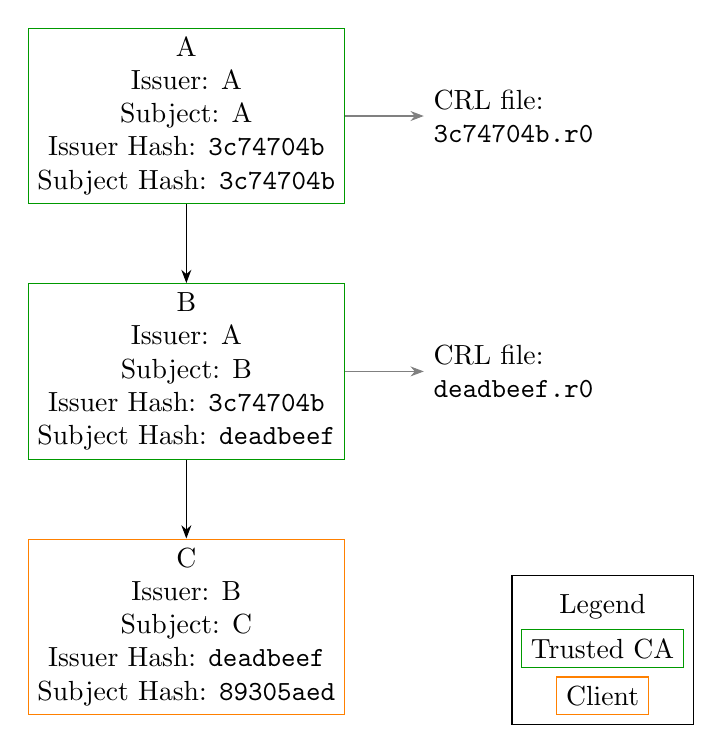
\begin{tikzpicture}
	% Styles.
	[ca/.style={rectangle,draw=green!60!black,minimum height=1cm,minimum width=1.5cm},
	leaf/.style={rectangle,draw=orange,minimum height=1cm, minimum width=1.5cm}]
	% Certificates.
	\node (A) at (0, 0) [ca,align=center] {A \\ Issuer: A \\ Subject: A \\ Issuer Hash: \texttt{3c74704b} \\ Subject Hash: \texttt{3c74704b}};
	\node (B) [below=of A] [ca,align=center] {B \\ Issuer: A \\ Subject: B \\ Issuer Hash: \texttt{3c74704b} \\ Subject Hash: \texttt{deadbeef}};
	\node (C) [below=of B] [leaf,align=center] {C \\ Issuer: B \\ Subject: C \\ Issuer Hash: \texttt{deadbeef} \\ Subject Hash: \texttt{89305aed}};
	\draw[-Stealth] (A) -- (B);
	\draw[-Stealth] (B) -- (C);
	\node (A CRL) [right=of A,align=left] {CRL file: \\ \texttt{3c74704b.r0}};
	\node (B CRL) [right=of B,align=left] {CRL file: \\ \texttt{deadbeef.r0}};
	\draw[-Stealth,gray] (A) -- (A CRL);
	\draw[-Stealth,gray] (B) -- (B CRL);
	% Legend.
	\node (lanchor) at (current bounding box.south east) {};
	\node (legend) at (lanchor) [above=1.1cm] {Legend};
	\node (l1) at (lanchor) [above=0.6cm,draw=green!60!black] {Trusted CA};
	\node (l2) at (lanchor) [above=0.0cm,draw=orange] {Client};
	\node [rectangle,draw,fit=(legend) (l1) (l2)] {};
\end{tikzpicture}
}
\end{makeimage}
\caption{Each CA requires its own CRL file.  The CRL file name is based on the hash of its issuer name.  Note that the \emph{issuer} of the CRL file is the \emph{subject} of its respective CA.}
\end{figure}
\end{center}

One more caveat: OpenSSL does not seem to report any error if the CRL path directory does not exist.  Figures.


% Syncing the Gentoo repository.
\section{2017-08-23 Securely Syncing the Gentoo Repository via a Local Server}

\begin{center}
\begin{figure}
\begin{makeimage}
\fbox{
\begin{tabular}{l|l}
Before: & After: \\
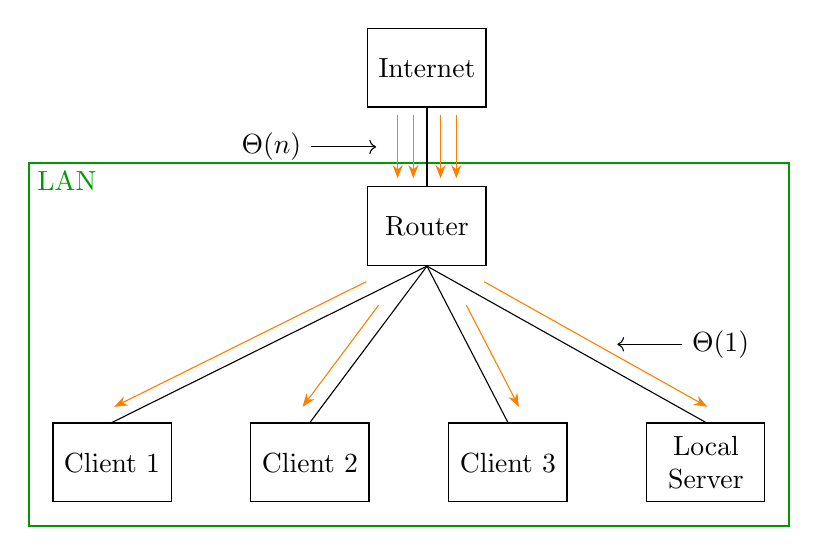
\begin{tikzpicture}
	% Machines.
	[puter/.style={rectangle,draw,minimum height=1cm,minimum width=1.5cm}]
	\node (client1)  at (0, 0) [puter] {Client 1};
	\node (client2)  [right=of client1] [puter] {Client 2};
	\node (client3)  [right=of client2] [puter] {Client 3};
	\node (server)   [right=of client3] [puter] {\parbox{1cm}{\centering Local \\ Server}};
	\node (router)   at (4, 3) [puter] {Router};
	\node (internet) [above=of router] [puter] {Internet};
	% Links.
	\draw (client1.north) -- (router.south)
		node[pos=0.1,left=0.2,circle](c1-r){}
		node[pos=0.9,left=0.2,circle](r-c1){};
	\draw (client2.north) -- (router.south)
		node[pos=0.1,left=0.07,circle](c2-r){}
		node[pos=0.75,left=0.07,circle](r-c2){};
	\draw (client3.north) -- (router.south)
		node[pos=0.1,right=0.07,circle](c3-r){}
		node[pos=0.75,right=0.07,circle](r-c3){};
	\draw (server.north) -- (router.south)
		node[pos=0.1,right=0.2,circle](s-r){}
		node[pos=0.9,right=0.2,circle](r-s){}
		node[pos=0.5,right=0.3,circle](smid){};
	\draw (router.north) -- (internet.south)
		node[pos=0.1,left=0.2,circle](r1-i1){}
		node[pos=0.1,left=0,circle](r2-i2){}
		node[pos=0.1,right=0,circle](r3-i3){}
		node[pos=0.1,right=0.2,circle](r4-i4){}
		node[pos=0.9,left=0.2,circle](i1-r1){}
		node[pos=0.9,left=0,circle](i2-r2){}
		node[pos=0.9,right=0,circle](i3-r3){}
		node[pos=0.9,right=0.2,circle](i4-r4){}
		node[pos=0.5,left=0.3,circle](mid){};
	% Traffic.
	\draw[orange,-Stealth] (r-c1.center) -- (c1-r.center);
	\draw[orange,-Stealth] (r-c2.center) -- (c2-r.center);
	\draw[orange,-Stealth] (r-c3.center) -- (c3-r.center);
	\draw[orange,-Stealth] (r-s.center) -- (s-r.center);
	\draw[orange,-Stealth] (i1-r1.center) -- (r1-i1.center);
	\draw[orange,-Stealth] (i2-r2.center) -- (r2-i2.center);
	\draw[orange,-Stealth] (i3-r3.center) -- (r3-i3.center);
	\draw[orange,-Stealth] (i4-r4.center) -- (r4-i4.center);
	\draw [<-] (mid) -- +(-1, 0) node[left]{$\Theta(n)$};
	\draw [<-] (smid) -- +(1, 0) node[right]{$\Theta(1)$};
	% LAN box.
	\begin{scope}[on background layer]
		\node (bback) [rectangle,thick,draw=green!60!black,inner sep=0.3cm,fit=(client1) (server) (router)] {};
		\node [below right,text=green!60!black] at (bback.north west) {LAN};
	\end{scope}
\end{tikzpicture}
&  % Copy+paste'd
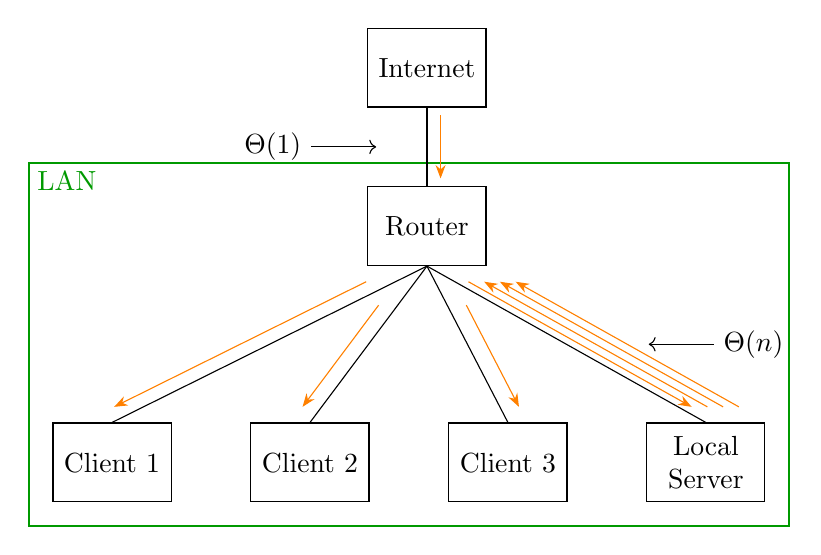
\begin{tikzpicture}
	% Machines.
	[puter/.style={rectangle,draw,minimum height=1cm,minimum width=1.5cm}]
	\node (client1)  at (0, 0) [puter] {Client 1};
	\node (client2)  [right=of client1] [puter] {Client 2};
	\node (client3)  [right=of client2] [puter] {Client 3};
	\node (server)   [right=of client3] [puter] {\parbox{1cm}{\centering Local \\ Server}};
	\node (router)   at (4, 3) [puter] {Router};
	\node (internet) [above=of router] [puter] {Internet};
	% Links.
	\draw (client1.north) -- (router.south)
		node[pos=0.1,left=0.2,circle](c1-r){}
		node[pos=0.9,left=0.2,circle](r-c1){};
	\draw (client2.north) -- (router.south)
		node[pos=0.1,left=0.07,circle](c2-r){}
		node[pos=0.75,left=0.07,circle](r-c2){};
	\draw (client3.north) -- (router.south)
		node[pos=0.1,right=0.07,circle](c3-r){}
		node[pos=0.75,right=0.07,circle](r-c3){};
	\draw (server.north) -- (router.south)
		node[pos=0.1,right=0,circle](s-r){}
		node[pos=0.9,right=0,circle](r-s){}

		node[pos=0.1,right=0.2,circle](s-c1){}
		node[pos=0.9,right=0.2,circle](c1-s){}
		node[pos=0.1,right=0.4,circle](s-c2){}
		node[pos=0.9,right=0.4,circle](c2-s){}
		node[pos=0.1,right=0.6,circle](s-c3){}
		node[pos=0.9,right=0.6,circle](c3-s){}

		node[pos=0.5,right=0.7,circle](smid){};
	\draw (router.north) -- (internet.south)
		node[pos=0.9,right=0,circle](i-s){}
		node[pos=0.1,right=0,circle](s-i){}
		node[pos=0.5,left=0.3,circle](mid){};
	% Traffic.
	\draw[orange,-Stealth] (r-c1.center) -- (c1-r.center);
	\draw[orange,-Stealth] (r-c2.center) -- (c2-r.center);
	\draw[orange,-Stealth] (r-c3.center) -- (c3-r.center);
	\draw[orange,-Stealth] (r-s.center) -- (s-r.center);
	\draw[orange,-Stealth] (s-c1.center) -- (c1-s.center);
	\draw[orange,-Stealth] (s-c2.center) -- (c2-s.center);
	\draw[orange,-Stealth] (s-c3.center) -- (c3-s.center);
	\draw[orange,-Stealth] (i-s.center) -- (s-i.center);
	\draw [<-] (mid) -- +(-1, 0) node[left]{$\Theta(1)$};
	\draw [<-] (smid) -- +(1, 0) node[right]{$\Theta(n)$};
	% LAN box.
	\begin{scope}[on background layer]
		\node (bback) [rectangle,thick,draw=green!60!black,inner sep=0.3cm,fit=(client1) (server) (router)] {};
		\node [below right,text=green!60!black] at (bback.north west) {LAN};
	\end{scope}
\end{tikzpicture}
\end{tabular}
}
\end{makeimage}
\caption{Using a local server for the Gentoo repository takes pressure off of the (often relatively slow) Internet connection and places it onto the (often relatively fast) LAN, especially important for those whose Internet is metered.}
\end{figure}
\end{center}

Running multiple Gentoo machines normally means keeping a copy of the Gentoo repository on each machine; by default this also means updating each copy of the repository by having each machine call out to the Gentoo mirrors on a regular basis for updates.  This is a waste of both local and upstream bandwidth and resources, because, within a given time period, the repository is the exact same regardless of the type of machine it is on; instead, it is more efficient to set up one machine as a server that synchronizes with upstream, then have the other local machines synchronize to said local server.  This guide will explain how to do that securely.

Though there are multiple protocols that Portage can use for synchronization, this guide will cover only SSH, and \texttt{rsync+stunnel}.  Both of these are secure, allowing synchronization over an untrusted network, albeit the local server must be trusted.  Securely syncing the server to the upstream repository with \texttt{FEATURES=webrsync-gpg} is not covered here, as it is instead covered \htmladdnormallink{here}{https://wiki.gentoo.org/wiki/Handbook:AMD64/Working/Features#Validated_Gentoo_repository_snapshots}.

\subsection{SSH Synchronization}
One of the pros of SSH-based synchronization is that it requires no extra server configuration for machines that already have SSH access to the server.  The downside is that SSH access means shell access, which might not be desirable if any of the local machines is not fully trusted, for example, because it is running proprietary applications for, say, video games; one could try and circumvent this potential security weakness by giving the SSH user a restricted shell such as \texttt{rssh}, but I was unable to get \texttt{rssh} working with the \texttt{rsync} arguments that Portage wanted to use (note: Portage calls \texttt{rsync} over the SSH session).  Thus I prefer \texttt{rsync+stunnel}, but am including the SSH method for completeness and possible future reference.
\subsubsection{Server} Assuming that \texttt{sshd} is already set up (find one of many guides if it is not), the only thing that may need to be done is to add a special user for synchronization.  In order to add the user, run
\begin{quote}
\begin{verbatim}
	# useradd -m -s /bin/bash rsyncuser
	# passwd rsyncuser
\end{verbatim}
\end{quote}
\ldots then edit the SSH daemon configuration file, usually \texttt{/etc/ssh/sshd_config}, to contain the following line:
\begin{quote}
\begin{verbatim}
	AllowUsers rsyncuser
\end{verbatim}
\end{quote}
Depending on the selected authentication method for SSH, this may be enough to give the user access; however, in the case that only key-based authentication is allowed (usually via something like \texttt{PasswordAuthentication no} \& \texttt{ChallengeResponseAuthentication no} in \texttt{sshd_config}) an SSH keypair will need to be generated for the user and the private key copied to each client that wishes to synchronize with the server.  This can be done with the following commands:
\begin{quote}
\begin{verbatim}
	# cd /home/rsyncuser
	# su rsyncuser
	$ umask 0066
	$ mkdir -p .ssh
	$ ssh-keygen -a 16 -t ed25519
	$ cp .ssh/id_ed25519.pub .ssh/authorized_keys
\end{verbatim}
\end{quote}
This will create a keypair for the \texttt{rsyncyser} and authorize that keypair for SSH login.  The \texttt{.ssh/id_ed25519} file (the private key) will then need to be copied to the client machines, probably via a USB storage device:
\begin{quote}
\begin{verbatim}
	# cp .ssh/id_ed25519 /path/to/probably/usb/storage/device
\end{verbatim}
\end{quote}

This ends the server-side configuration.

\subsubsection{Clients}
By default, Portage knows how to use SSH for synchronization, so basic setup is quite simple, although some of the details are rather esoteric.

In order to tell Portage to synchronize over SSH, if it hasn't been done already, set up the main repository configuration via:
\begin{quote}
\begin{verbatim}
	# mkdir -p /etc/portage/repos.conf
	# cp /usr/share/portage/config/repos.conf /etc/portage/repos.conf/gentoo.conf
\end{verbatim}
\end{quote}
This creates, at the time of this writing, at least, a sane configuration file for the default repository that can then be reconfigured.  With this file created, Portage should function as it always has; the defaults must be overridden in order to actually change its behavior. In order to use SSH, edit the \texttt{/etc/portage/repos.conf/gentoo.conf} file by changing the \texttt{sync-uri} option under the \texttt{[gentoo]} section to read:
\begin{quote}
\begin{verbatim}
	sync-uri = ssh://rsyncuser@192.168.1.1/usr/portage
\end{verbatim}
\end{quote}
\ldots where \texttt{192.168.1.1} is replaced with the network address of the local server.  Portage will now begin trying to sync via SSH.

"Trying" may be the modus operandi depending on whether or not the local server strictly requires keys or will accept user passwords; it is thus useful to understand where Portage stores its SSH information, as its home directory is not \texttt{/home/portage}, but, as \texttt{/etc/passwd} reveals, \texttt{/var/tmp/portage}, thus SSH configuration goes into \texttt{/var/tmp/portage/.ssh}.  In order to get Portage to use \texttt{rsyncuser}'s key, run the following:
\begin{quote}
\begin{verbatim}
	# mkdir -p /var/tmp/portage/.ssh
	# umask 0066
	# cp /path/from/probably/usb/device/with/rsyncusers/key/id_ed25519 /var/tmp/portage/.ssh/id_ed25519
	# chown -R portage:portage /var/tmp/portage/.ssh
\end{verbatim}
\end{quote}
Portage should now pickup \texttt{rsyncuser}'s key when it tries to synchronize.

Admittedly, storing valuable authentication information in a \texttt{/var/tmp} subdirectory seems risky at best.  Another option for storing the key is to place the key at a more stable location and then tell Portage where to find it.  Start by placing the key somewhere safer:
\begin{quote}
\begin{verbatim}
	# mkdir -p /usr/local/portage/.ssh
	# chmod 700 /usr/local/portage/.ssh
	# chown -R portage:portage /usr/local/portage/.ssh
	# mv /var/tmp/portage/.ssh/id_ed25519 /usr/local/portage/.ssh/
\end{verbatim}
\end{quote}
\ldots then tell Portage where to find the key by adding the following line to \texttt{/etc/portage/make.conf}:
\begin{quote}
\begin{verbatim}
	PORTAGE_SSH_OPTS="-i /usr/local/portage/.ssh/id_ed25519"
\end{verbatim}
\end{quote}
Portage will now look for the \texttt{rsyncuser}'s key at the previously-specified location.

This solves the \texttt{rsyncuser}'s key problem, but what about the important \texttt{known_hosts} file?  Well, I didn't get that far.  I don't fully trust of all my machines, and do not want to give all of them shell access to my server, and, since I couldn't get \texttt{rssh} to work with Portage and was looking for an excuse to play with \texttt{stunnel}, I decided to work on it instead, thus \texttt{rsync+stunnel} is the topic of the next section.

\subsection{Rsync+stunnel Synchronization}
This method works by using an \texttt{rsync} daemon to synchronize between the local server and client; however, because \texttt{rsync} is unencrypted, the connection is wrapped via the \texttt{stunnel} daemon, which uses \htmladdnormallink{TLS}{https://en.wikipedia.org/wiki/Transport_Layer_Security} for encryption and authentication.  \texttt{stunnel} must be configured on both the local server and each client.

\subsubsection{Server}
Start by setting up the \texttt{rsync} daemon without \texttt{stunnel}.  By default, Gentoo comes with a disabled but sane configuration file at \texttt{/etc/rsyncd.conf}.  Adding a few extra lines gives, excluding comments, the following:
\begin{quote}
\begin{verbatim}
	pid file = /run/rsyncd.pid
	use chroot = yes
	read only = yes
	hosts allow = 192.168.1.1/16
	reverse lookup = no
	timeout = 60

	[gentoo-portage]
	path = /usr/portage
	comment = Gentoo Portage tree
	exclude = /distfiles /packages
\end{verbatim}
\end{quote}
By default this configuration file creates an \texttt{rsync} \textit{module} that clients can synchronize with; this module is read-only and excludes directories that are not a part of the repository.  The extra options are: \texttt{hosts allow = 192.168.1.1/16}, which tells \texttt{rsync} to only accept connections from hosts in the specified block and must be appropriate to the local network; \texttt{reverse lookup = no}, which disables reverse-DNS lookups of client IP addresses; and \texttt{timeout = 60}, which sets a small timeout for unresponsive clients.  See \texttt{man 5 rsyncd.conf} for details; the extra options are not strictly necessary for the purposes of this guide.

The next step is to install and configure \texttt{stunnel}.  This involves four steps: installing the program, configuring the service, generating certificates, and creating the service: To install \texttt{stunnel}, run:
\begin{quote}
\begin{verbatim}
	# emerge -av stunnel
\end{verbatim}
\end{quote}
For convenience, the Gentoo developers created a useful example configuration file for \texttt{rsync+stunnel} which may be installed by running:
\begin{quote}
\begin{verbatim}
	USE="stunnel" emerge -av rsync
\end{verbatim}
\end{quote}
This creates the file \texttt{/etc/stunnel/rsyncd.conf}.  Move it to \texttt{/etc/stunnel/rsyncd-stunnel.conf} for \texttt{init} scripts (later), and reconfigure it such that, excluding comments, it has the following options:
\begin{quote}
\begin{verbatim}
	foreground = no
	pid = /var/run/stunnel/rsyncd-stunnel.pid
	socket = l:TCP_NODELAY=1
	socket = r:TCP_NODELAY=1
	setuid = root
	setgid = root

	[rsync]
	accept = 874
	cert = /etc/stunnel/rsyncd-stunnel.crt
	key  = /etc/stunnel/rsyncd-stunnel.key
	client = no

	exec = /usr/bin/rsync
	execargs = rsync --server --daemon --config=/etc/rsyncd.conf .
\end{verbatim}
\end{quote}
Most of these options come with the default configuration file, but make sure to change the \texttt{pid} option.  The \texttt{cert} and \texttt{key} options specify where the \htmladdnormallink{X.509}{https://en.wikipedia.org/wiki/X.509} certificate and its key are to be loaded from (they will be generated later).  Port \texttt{874} is used in place of \texttt{873}, as it is not a plaintext \texttt{rsync} service.  Client verification is not wanted here, so make sure to remove any \texttt{verify} and \texttt{CAfile} lines.

In order to generate the server's certificate, run the following series of commands:
\begin{quote}
\begin{verbatim}
	# cd /etc/stunnel
	# umask 0077
	# openssl genrsa -out rsyncd-stunnel.key 4096
	# openssl req -key rsyncd-stunnel.key -new -x509 -days 7200 -sha512 -out rsyncd-stunnel.crt -subj '/CN=rsyncd-stunnel/'
\end{verbatim}
\end{quote}
The short story here is that this will create a certificate and key pair for TLS that will last for almost 20 years, see \texttt{man genrsa} and \texttt{man req} for details.

Finally, create the service with:
\begin{quote}
\begin{verbatim}
	# cd /etc/init.d
	# ln -s stunnel rsyncd-stunnel
\end{verbatim}
\end{quote}
This uses the default \texttt{stunnel} init script, except it will look for a configuration file at \texttt{/etc/stunnel/rsyncd-stunnel.conf}, hence the earlier renaming that was done.  To start the service, run \texttt{rc-service rsyncd-stunnel start}, and don't forget to add it to the default runlevel via:
\begin{quote}
\begin{verbatim}
	# rc-update add rsyncd-stunnel default
\end{verbatim}
\end{quote}

The server should now be configured and ready for synchronization.  The clients must now be configured to trust and use the server.

\subsubsection{Clients}
The client must now be configured so that when Portage attempts to sync it will use the secure connection \textbf{and} it will validate that it is syncing with the server, otherwise a malicious actor could imitate the server and send a compromised repository.  This involves installing and configuring \texttt{stunnel}, configuring Portage, then creating the service.

Begin by installing \texttt{stunnel}:
\begin{quote}
\begin{verbatim}
	# emerge -av stunnel
\end{verbatim}
\end{quote}
\ldots then configure \texttt{stunnel} so that, without comments, the configuration file \texttt{/etc/stunnel/stunnel.conf} reads:
\begin{quote}
\begin{verbatim}
	setuid = stunnel
	setgid = stunnel
	pid = /run/stunnel/stunnel.pid
	socket = l:TCP_NODELAY=1
	socket = r:TCP_NODELAY=1

	[rsync-stunnel]
	client     = yes
	CAfile     = /etc/stunnel/rsyncd-stunnel.crt
	verifyPeer = yes
	accept     = 127.0.0.1:873
	connect    = 192.168.1.200:874
\end{verbatim}
\end{quote}
This creates an \texttt{stunnel} \emph{service}.  The \texttt{client} argument lets \texttt{stunnel} know to run \texttt{rsync} as a client rather than as a server.  The \texttt{CAfile} argument specifies the location of the server certificate to use (note that it has not yet been copied over to the client).  The \texttt{verifyPeer} is especially important as enabling it will actually validate the server certificate; without this enabled a malicious actor could intercept and modify the traffic.  The \texttt{accept} argument specifies where the \texttt{stunnel} program will listen for client connections, Portage will later be configured to make connections here.  The \texttt{connect} argument specifies where the \texttt{stunnel} program will connect to; it must be set to the address and port of the local server.  The other options are fairly standard.  Note that, unlike the server, this setup is using the default \texttt{stunnel} settings, configuring multiple \texttt{stunnel} services at the OpenRC level would require modifying a few parameters, such as the PID (Process ID) and the filename of the configuration.

Now that \texttt{stunnel} has been configured, make sure to copy the certificate from the local server to the client.  This should be done via a trusted storage device (USB stick, SD Card, \&c.) or the certificate retrieved via a command such as OpenSSL's \texttt{s\_client} (usage not covered here) and its fingerprint manually verified.
\begin{quote}
\begin{verbatim}
	# cp /path/from/secure/storage/device /etc/stunnel/rsyncd-stunnel.crt
\end{verbatim}
\end{quote}
\texttt{stunnel} now has all that it needs to securely tunnel a connection to the server.

Portage must now be configured to use the secure tunnel.  As with SSH configuration, begin by overriding the default repository configuration:
\begin{quote}
\begin{verbatim}
	# mkdir -p /etc/portage/repos.conf
	# cp /usr/share/portage/config/repos.conf /etc/portage/repos.conf/gentoo.conf
\end{verbatim}
\end{quote}
\ldots then modify the \texttt{sync-uri} argument to correspond to the \texttt{accept} argument configured in \texttt{stunnel}:
\begin{quote}
\begin{verbatim}
	sync-uri = rsync://127.0.0.1:873/gentoo-portage
\end{verbatim}
\end{quote}
This will synchronize with the \texttt{gentoo-portage} module defined on the local server's \texttt{/etc/rsyncd.conf}.  Note how the use of \texttt{stunnel} is completely transparent to Portage.  This has the minor disadvantage that error diagnostics must be found in log message from \texttt{stunnel} and not the Portage frontend, but is usually not a problem once things have been configured properly.

Next, start the service and add it to the default runlevel:
\begin{quote}
\begin{verbatim}
	# rc-service stunnel start
	# rc-update add stunnel default
\end{verbatim}
\end{quote}
\ldots then try it out with:
\begin{quote}
\begin{verbatim}
	# emerge --sync
\end{verbatim}
\end{quote}
Portage should now be securely synchronizing to the local server!  Repeat these steps for each client that needs to synchronize with the local server.


% Ancient Apparition Bowling
\section{2017-07-17 Ancient Apparition Bowling}
This is a silly metagame that I came up with for a DotA2 custom game.  It may not be possible to beat, but I've yet to try all strategies.

\subsection*{Origin}
Mercilessly slaughtering bots using weird combinations of cheats in DotA2 is an easy way to blow off a little steam after a difficult match.  One day I decided to go "bowling" with Ancient Apparition; I'd cheat to maximum level, 6-slot, enable wtf mode, and snipe the bots from base with his ultimate.
This is loads of fun, until the creeps start pushing towers, at which point the bots also take advantage of wtf mode and begin spamming fortify, leading to a frustrating stalemate.  The workaround for this is to disable wtfmode and instead use the \texttt{-refresh} cheat, which, although it does reset fortify cooldowns, can be used in conjunction with a Refresher Orb to blast the bots with two ultimates while giving them only one fortify.

The result is a semi-functional slaughtering of bots, although having to constantly open the command prompt to paste and submit the \texttt{-refresh} command gets annoying after a while; sadly, there doesn't seem to be a way to disable the bots' fortify spam.  After a little bit of this, I noticed that the cooldown of the metaphorical bowling ball and the travel time were not that far apart, leading me to wonder if I could play this game successfully without having to spam cheat commands (and reset the fortify cooldown) all game long.  Thus "Ancient Apparition Bowling" was born.

\subsection*{Rules}
These are the rules of the game, and though they may not be comprehensive, you should be able to understand the jist of them.  First, stay in fountain for the duration of the match.  Second, use cheats to give yourself max level (\texttt{-lvlup 25}), 6-slots (\texttt{-item <name>}), and vision (\texttt{-allvision}).  Third, no backpack, stash, or other item-use shenanegains; stick to your 6 slots. (TODO: pic of fountain)  Fourth, no bots on your team and five bots of highest difficulty on the other team.  That's it!
\begin{figure}

\includegraphics[scale=0.33]{files/blog/2017_07_17_ancient_apparition_bowling/fountain.png}
\caption{Where you will be spending all of your time.}
\end{figure}

Your goal is now to destroy the bots' ancient before the bots level up enough to tank through your ult and push your base.  This is more difficult than it sounds, as the bots are actually rather crafty and level up sooner than you might expect.

\subsection*{Strategy}
My current build involves getting an Aghaim's Scepter, Octarine Core, Refresher Orb, and 3 Aether Lens (TODO: picture of items).  Perhaps you can think up something better.
\begin{figure}

\includegraphics{files/blog/2017_07_17_ancient_apparition_bowling/items.png}
\end{figure}

It is difficult to push all lanes at once, since the bots can quickly respawn at lower levels, and you only have so many ultimates to shoot off.  It would thus seem prudent to choose a particular lane to hammer, but how to do so isn't actually obvious.

The strategy that I tried was to focus the enemy creeps at their spawning point in a side lane.  This can be done by firing consistently at the 18 and 48 second marks towards the front of their 3rd tower. This will obliterate all of the creeps during the early part of the game.  Make sure to adjust your ultimate slightly to the left each time in order to adjust for the micro-delay between your ult going off cooldown and actually launching your ult; you can reset this after a while with a Refresher Orb.
\begin{figure}
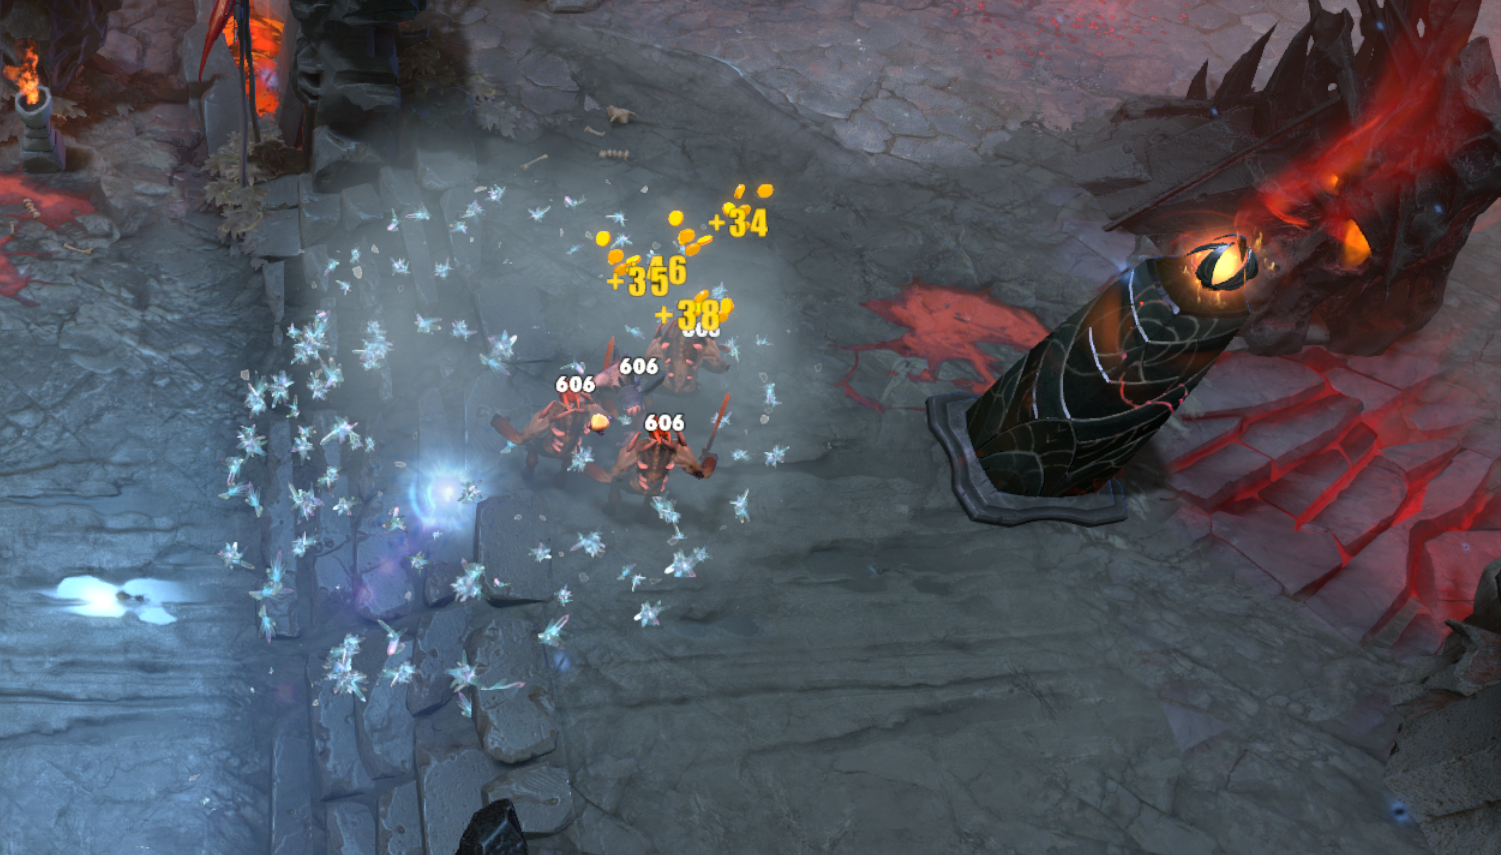
\includegraphics[scale=0.33]{files/blog/2017_07_17_ancient_apparition_bowling/towerhit.png}
\caption{Killing creeps as soon as they spawn.}
\end{figure}

Though this may at first seem like a good way to get the creeps to push the tower, the bots are actually crafty enough to pull the creeps behind the tower, limiting the amount of damage done.  While I was able to eventually push to their barracks, at this point the other bots also helped pull the creeps behind the barracks, and eventually became strong enough to tank the ult and push my base, thus making this a losing strategy.
\begin{figure}
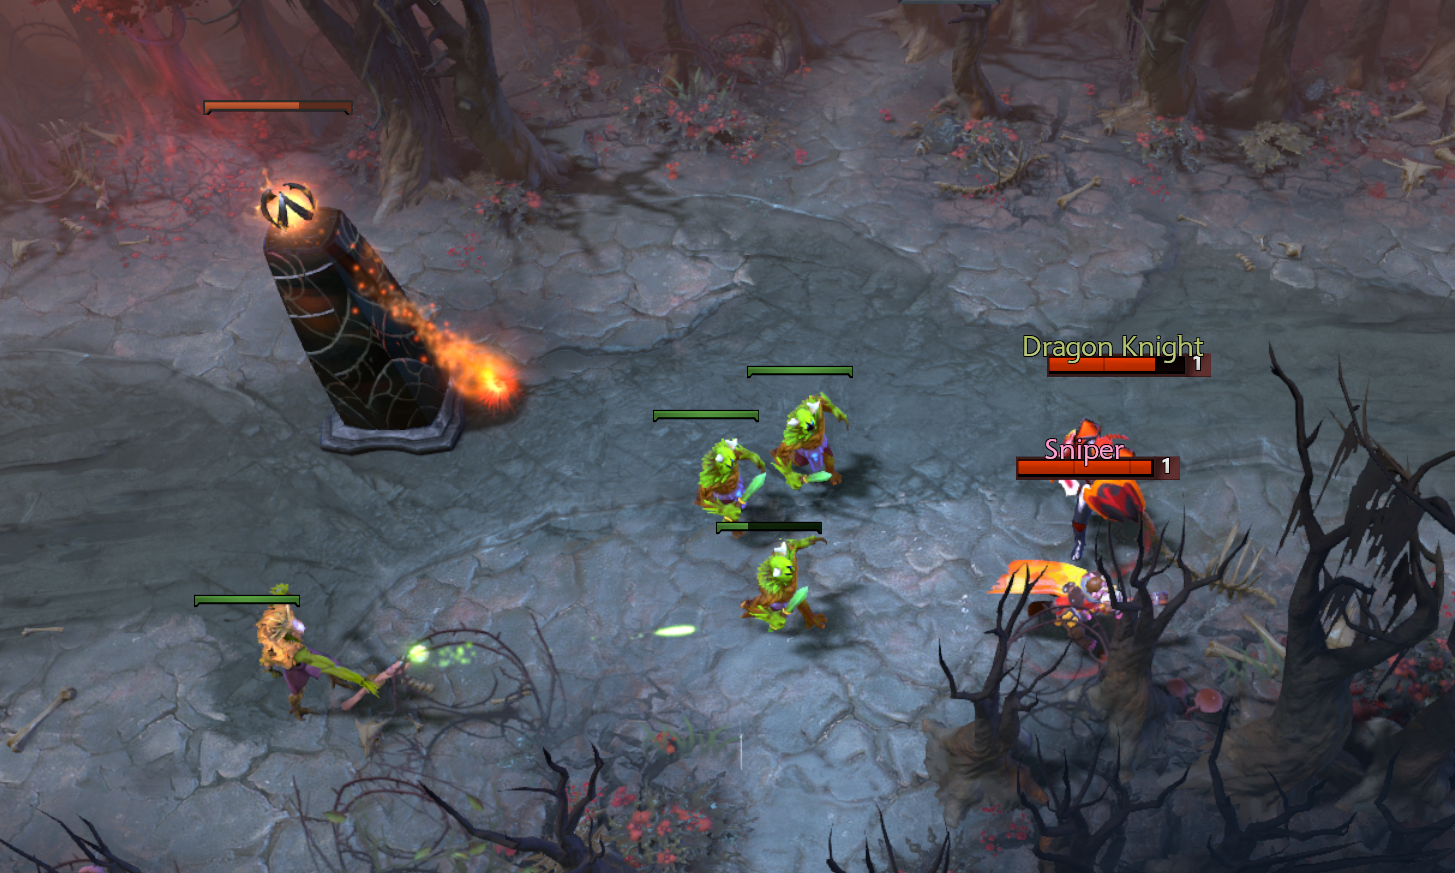
\includegraphics[scale=0.33]{files/blog/2017_07_17_ancient_apparition_bowling/botpull.png}
\caption{Sneaky bots pulling creeps away from the tower.}
\end{figure}

A possible variation would be to try focusing down the bots themselves, but this is tricky as they often move out of the ult's way.  A hybrid combination may involve finding a position where the bots and creeps are likely to align, then aiming to kill the creeps and probably the bots.  It may also be easier to push straight up middle rather than taking out a side lane first, especially as the bots seem found of charging up mid.

I've yet to win at this metagame.  It might not even be plausible.  Try it yourself and see what happens!

\subsection*{Addendum}
Between inventing this game, writing this article, and getting the screenshots, the bot fortify spam in wtf mode seems to have stopped.

\end{document}
